%%s Beamer template was created by Cameron Bracken.
%%  Anyone can freely use or modify it for any purpose
%%  without attribution.
%%
%%  Last Modified: January 9, 2009
%%

\documentclass[xcolor=x11names,compress]{beamer}

%% General document %%%%%%%%%%%%%%%%%%%%%%%%%%%%%%%%%%
\usepackage{graphicx}
\usepackage{tikz}
\usetikzlibrary{decorations.fractals}
%%%%%%%%%%%%%%%%%%%%%%%%%%%%%%%%%%%%%%%%%%%%%%%%%%%%%%

%% Color Definitions%%%%%%%%%%%%%%%%%%%%%%%%%%%%%%%%%%
\definecolor{pinegreen}{rgb}{0.0, 0.47, 0.44}
\definecolor{charcoal}{rgb}{0.21, 0.27, 0.31}
\definecolor{viridian}{rgb}{0.25, 0.51, 0.43}
\definecolor{rust}{rgb}{0.72, 0.25, 0.05}
\definecolor{taupegray}{rgb}{0.55, 0.52, 0.54}
\definecolor{tomato}{rgb}{1.0,  0.38823529,  0.27843137}
\definecolor{dodgerblue}{rgb}{0.11764706,  0.56470588,  1.0}
\definecolor{darkcoral}{rgb}{0.8, 0.36, 0.27}
%%%%%%%%%%%%%%%%%%%%%%%%%%%%%%%%%%%%%%%%%%%%%%%%%%%%%%


%% Beamer Layout %%%%%%%%%%%%%%%%%%%%%%%%%%%%%%%%%%
\useoutertheme[subsection=false,shadow]{miniframes}
\useinnertheme{default}
%\usefonttheme{serif}
\usepackage[sfdefault,light]{roboto}  %% Option 'sfdefault' only if the base font of the document is to be sans serif
\usepackage[T1]{fontenc}
\usepackage{palatino}
\usepackage{braket}
\setbeamertemplate{navigation symbols}{}
\setbeamertemplate{footline}[frame number]
\setbeamerfont{title like}{shape=\scshape}
\setbeamerfont{frametitle}{shape=\scshape}
\setbeamerfont{footnote}{size=\small}
\setbeamercolor*{lower separation line head}{bg=pinegreen}
\setbeamercolor*{normal text}{fg=black,bg=white}
\setbeamercolor*{alerted text}{fg=red}
\setbeamercolor*{example text}{fg=black}
\setbeamercolor*{structure}{fg=black}
\setbeamercolor*{palette tertiary}{fg=black,bg=black!5}
\setbeamercolor*{palette quaternary}{fg=black,bg=black!10}
\usepackage[listings,theorems]{tcolorbox}
%% Packages%%%%%%%%%%%%%%%%%%%%%%%%%%%%%%%%%%
\usepackage{soul}
\usepackage[style=chem-acs]{biblatex}
\bibliography{qmc_solids.bib}
\usepackage{listings}
%set up math font
\usepackage{amsmath}
\usepackage{mathpazo}
\renewcommand\rmdefault{lmr}
% all tikz packages for images
\usepackage{tikz}
\usepackage{tikzorbital}
\usetikzlibrary{arrows,shapes}
\tikzstyle{every picture}+=[remember picture]
\usepackage{graphicx}
% otherstuff
\usepackage{booktabs}
\usepackage{siunitx} % unit stuff
\usepackage{cancel} % to cross out stuff
\usepackage{modiagram}
\usepackage[version=3]{mhchem}
\usepackage{enumitem} % needed to have symbol in itemize in this template
\usepackage{array} %used for something in the template
\usepackage{hyperref} % url

%%%%%%%%%%%%%%%%%%%%%%%%%%%%%%%%%%%%%%%%%%%%%%%%%%%%%%

\renewcommand{\(}{\begin{columns}}
\renewcommand{\)}{\end{columns}}
\newcommand{\<}[1]{\begin{column}{#1}}
\renewcommand{\>}{\end{column}}

\title[{\makebox[.5\paperwidth]{General Chemistry Recitation 1\hfill
       \insertframenumber/\inserttotalframenumber}}]{ICE-T Day 1:\\
Introduction}
\author[\quad Amanda \quad\quad\quad\quad aed63@pitt.edu]{Amanda Dumi\\
dumia@duq.edu
}

\date{\small{\today}}


\begin{document}

%%%%%%%%%%%%%%%%%%%%%%%%%%%%%%%%%%%%%%%%%%%%%%%%%%%%%%
\section{Introduction}
\begin{frame}
\titlepage
\end{frame}
%%%%%%%%%%%%%%%%%%%%%%%%%%%%%%%%%%%%%%%%%%%%%%%%%%%%%%
%%%%%%%%%%%%%%%%%%%%%%%%%%%%%%%%%%%%%%%%%%%%%%%%%%%%%%
\begin{frame}{What are we going to do?}
    Make microbial fuel cells!
    \begin{center}
        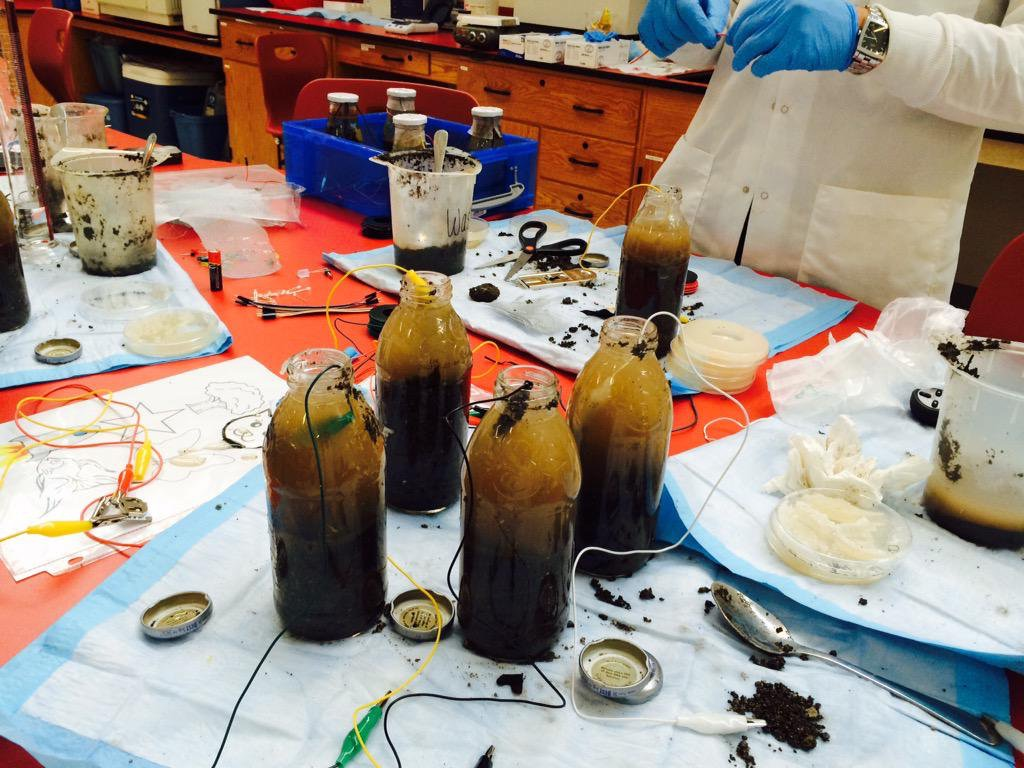
\includegraphics[width= 0.8\textwidth, height= 0.8\textheight, keepaspectratio]{fuelcell.jpg}
    \end{center}
\end{frame}
%%%%%%%%%%%%%%%%%%%%%%%%%%%%%%%%%%%%%%%%%%%%%%%%%%%%%%
%%%%%%%%%%%%%%%%%%%%%%%%%%%%%%%%%%%%%%%%%%%%%%%%%%%%%%
\begin{frame}{What are we going to do?}
    Learn to program in Python and Mathematica with a Raspberry Pi!
    \begin{center}
        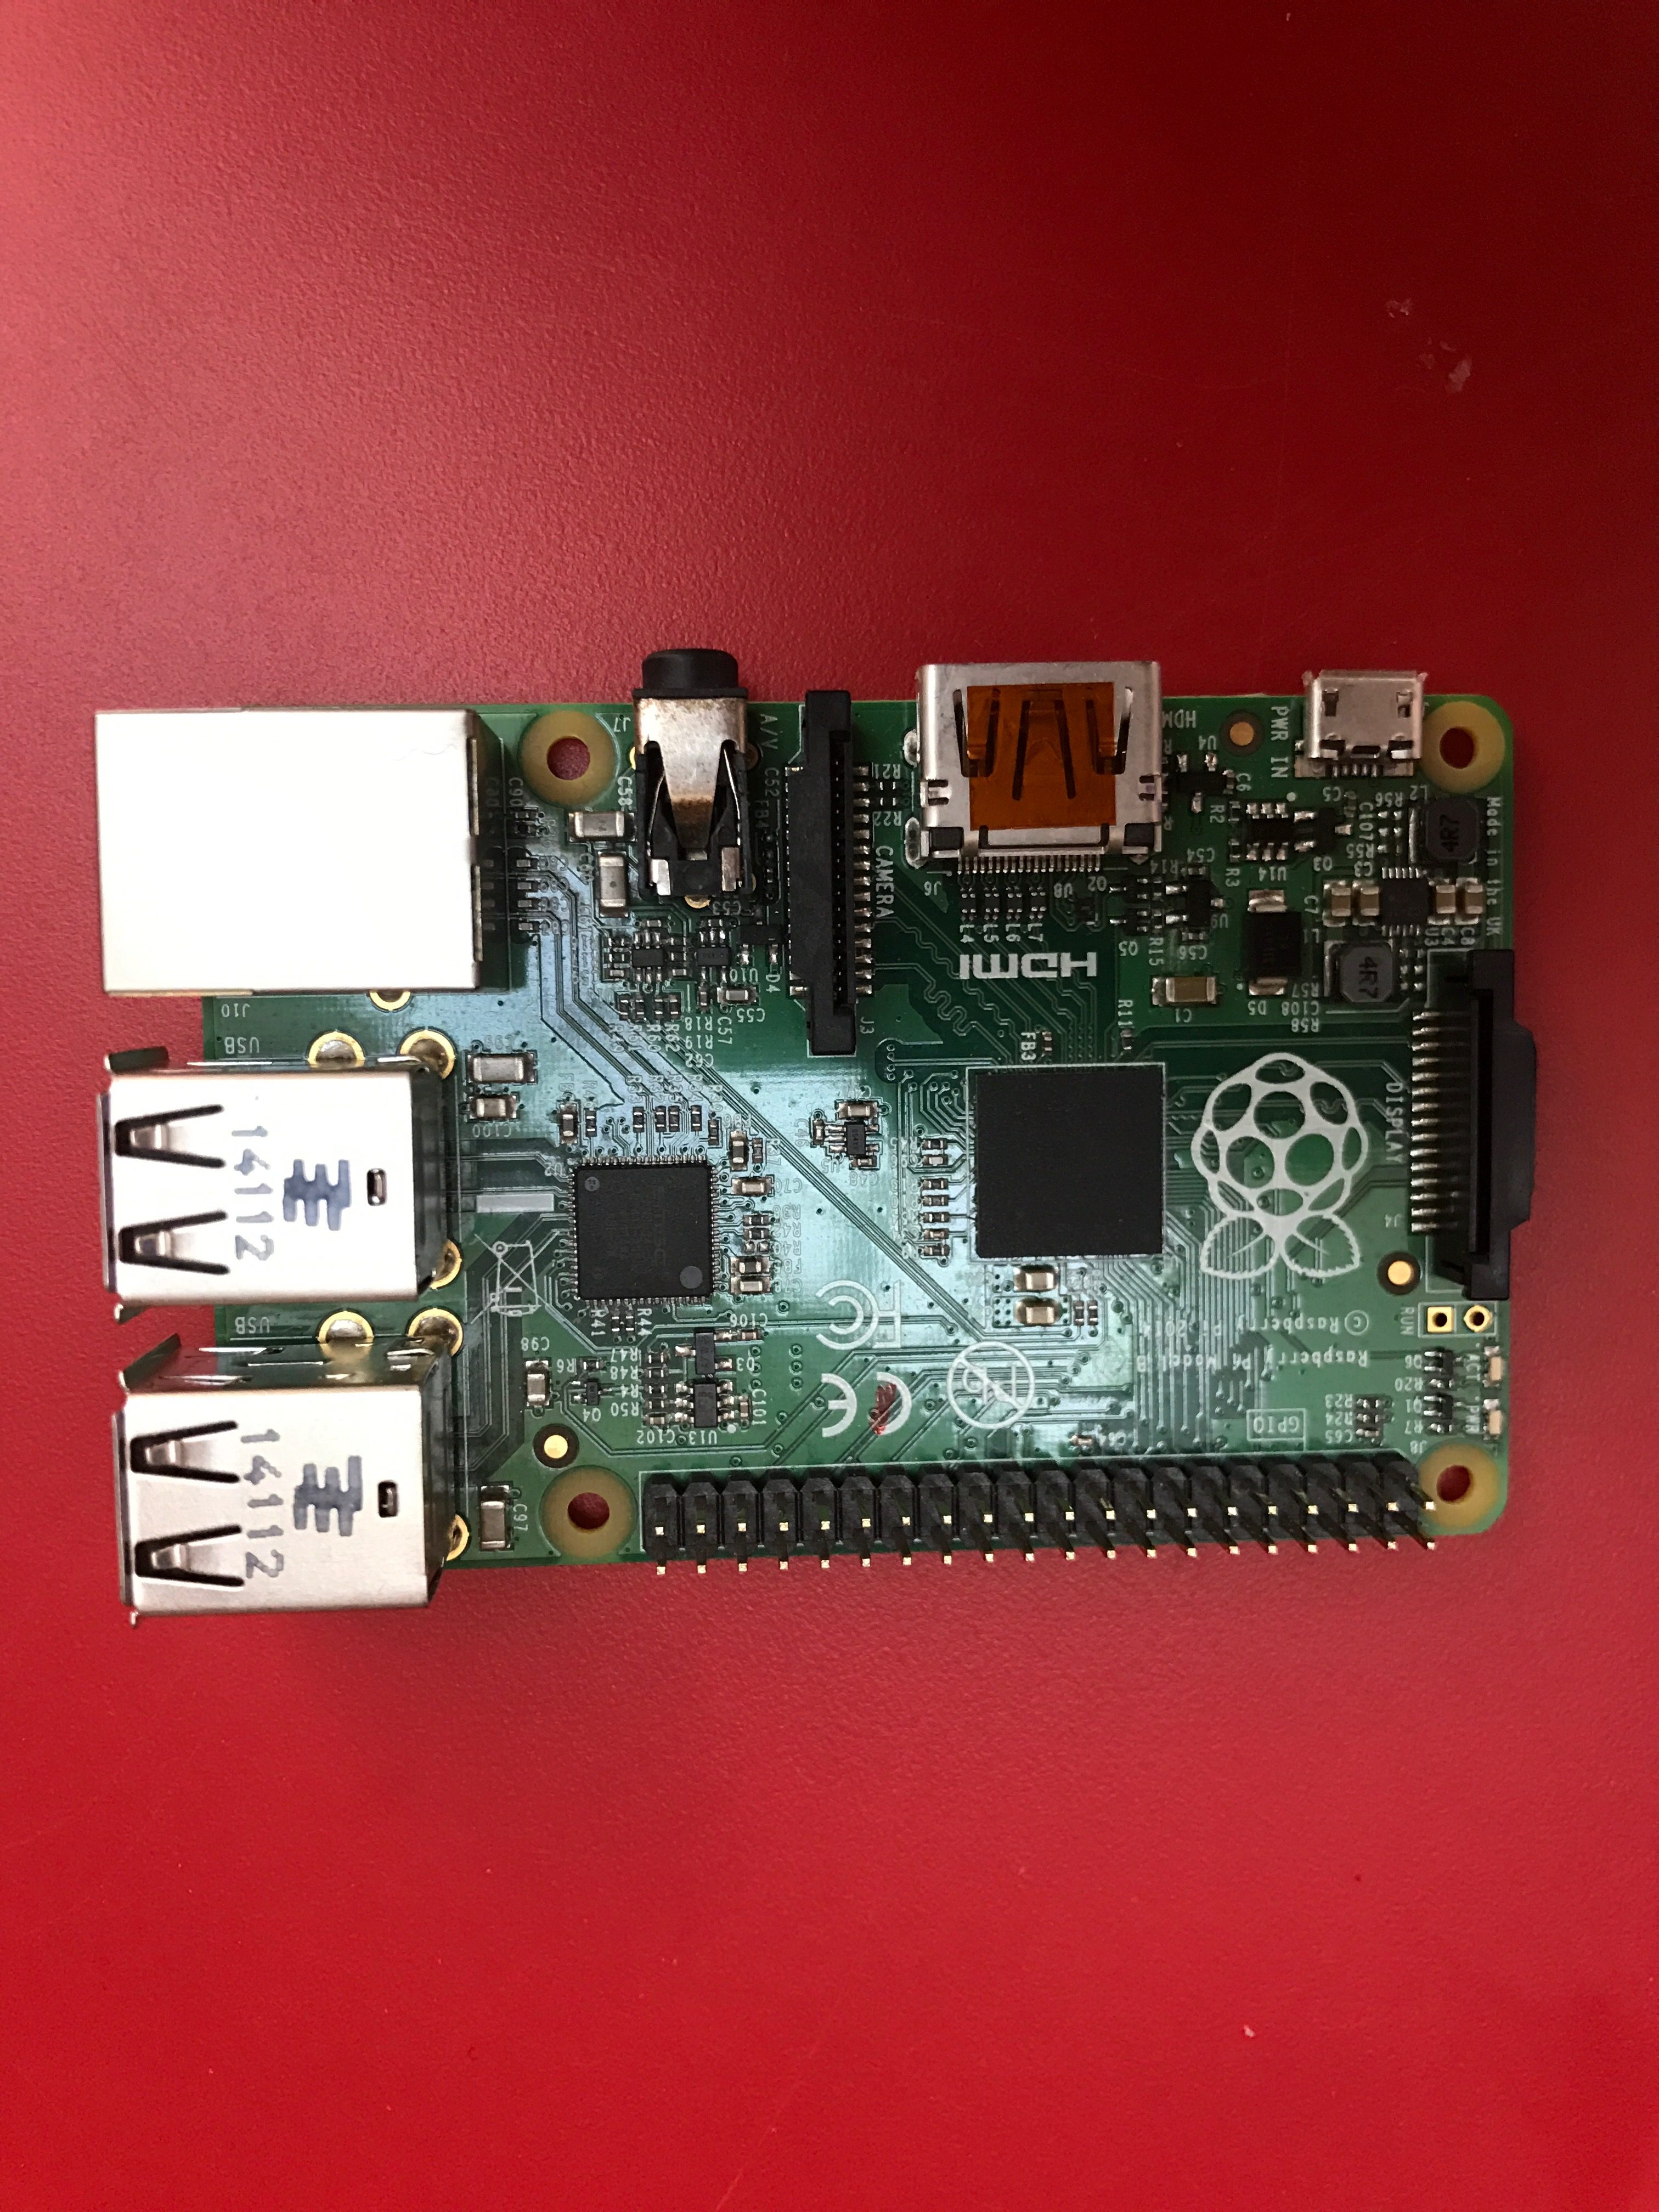
\includegraphics[width= 0.8\textwidth, height= 0.7\textheight, keepaspectratio]{raspberrypi.jpg}
    \end{center}
\end{frame}
%%%%%%%%%%%%%%%%%%%%%%%%%%%%%%%%%%%%%%%%%%%%%%%%%%%%%%
%%%%%%%%%%%%%%%%%%%%%%%%%%%%%%%%%%%%%%%%%%%%%%%%%%%%%%
    \begin{frame}{Why program?}
Programming allows us to...
\begin{enumerate}[label=$\bullet$]
\item \textcolor{darkcoral}{Data collection: } \textcolor{black}{automate data collection}  \vspace{0.5cm} \pause
\item \textcolor{darkcoral}{Data analysis:} \textcolor{black}{find trends in data we would otherwise miss} \vspace{0.5cm} \pause
\item \textcolor{darkcoral}{Data presentation:} \textcolor{black}{present our data in beautiful and informative ways}
\end{enumerate}
\end{frame}

%%%%%%%%%%%%%%%%%%%%%%%%%%%%%%%%%%%%%%%%%%%%%%%%%%%%%%
%%%%%%%%%%%%%%%%%%%%%%%%%%%%%%%%%%%%%%%%%%%%%%%%%%%%%%
\begin{frame}{Let's get started!}
    \begin{enumerate}[label=$\bullet$]
        \item \textcolor{darkcoral}{Put Kano together} \vspace{0.5cm} 
        \item \textcolor{darkcoral}{Try out Story Mode} \vspace{0.5cm} 
        \item \textcolor{darkcoral}{Try out Terminal Quest}
    \end{enumerate}
\end{frame}
%%%%%%%%%%%%%%%%%%%%%%%%%%%%%%%%%%%%%%%%%%%%%%%%%%%%%%
%%%%%%%%%%%%%%%%%%%%%%%%%%%%%%%%%%%%%%%%%%%%%%%%%%%%%%

\end{document}
